\section{Smart Manufacturing System and Data Environment}

This section establishes the operational foundation of the QASAMAP framework. This article begins with an overview of the three-tier architecture, then explains the data sources and their statistical characteristics, which form the basis for the design of predictive models, and finally details the data infrastructure and integration layer that enable real-time data delivery and model deployment.

\subsection{QASAMAP Architecture Overview}

QASAMAP is organized into three functional layers, as illustrated in Figure~\ref{fig:research_methodology}. The following paragraphs provide a high-level summary of each layer; subsequent subsections present detailed formulations and implementation specifics.

\textbf{Layer 1 Data and Predictive Modelling.} The first layer handles real-time sensor data ingestion via an Apache Kafka pipeline simulation and executes three families of predictive models. A Temporal Graph Convolutional Network (T-GCN) performs spatiotemporal sensor stream forecasting, exploiting a cross-correlation lag graph constructed from the temporal relationships among the 50 monitored machines. The cross-correlation graph comprises 50 nodes and 538 directed edges, with Machine 40 identified as the anchor node based on its highest out-degree centrality. Supervised tree-based ensemble models (XGBoost, LightGBM, CatBoost, HistGradientBoosting) and the TabNet deep tabular model are evaluated for five classification targets (machine status, anomaly flag, failure type, downtime risk, maintenance required) and one regression target (predicted RUL). The empirical motivation for graph-based modelling is grounded in the dataset: temperature (Pearson $r = 0.447$ with anomaly flag) is the most informative single sensor, and the cross-correlation structure reveals predictive relationships between machines that enable machine-wide anomaly propagation.

\textbf{Layer 2 Agentic AI Framework.} The second layer implements a multi-agent orchestration system comprising \textbf{nine} LLM-powered agents including Monitoring, Diagnosis, Planning, Reporting, Correlation, Explainability, Self-Reflection, Scheduling, and Pattern Learning coordinated by the Multi-Agent Orchestrator class using the "GLM LLM model" via the Ollama Cloud API. The LLM benchmark additionally evaluates "QWEN" and "DeepSeek" models. Each agent receives structured prompts containing classical risk context (risk score, sensor flags, RUL status) and quantum-inspired heuristic context (Pauli-Z labels, QUBO priority ranks, QAOA slot assignments). \textbf{Post-audit safeguard:} No ground-truth fields status, failure\_type) are passed to any LLM agent prompt. Supporting components include the ContextMemoryStore with sliding window and decision log, the ReasoningEngine for classical multi-factor risk scoring, and the LearningLoop for autonomous threshold adaptation based on false positive and false negative feedback.

\textbf{Layer 3 Quantum-Inspired Classical Heuristic Engine.} The third layer augments the agentic pipeline with three quantum-inspired classical heuristics: Pauli-Z multi-sensor risk encoding, QUBO-formulated priority ranking, and QAOA-formulated maintenance slot scheduling. Full mathematical formulations, algorithmic disclosures, and experimental assessment of these heuristics are presented in Chapter~\ref{chap:quantum}. A heuristic override mechanism escalates machines carrying quantum-style danger signals to active inspection even when their classical risk scores fall in the LOW category, providing a guard against false negatives that classical thresholds alone would miss.
\begin{figure}[!htbp]
    \centering
    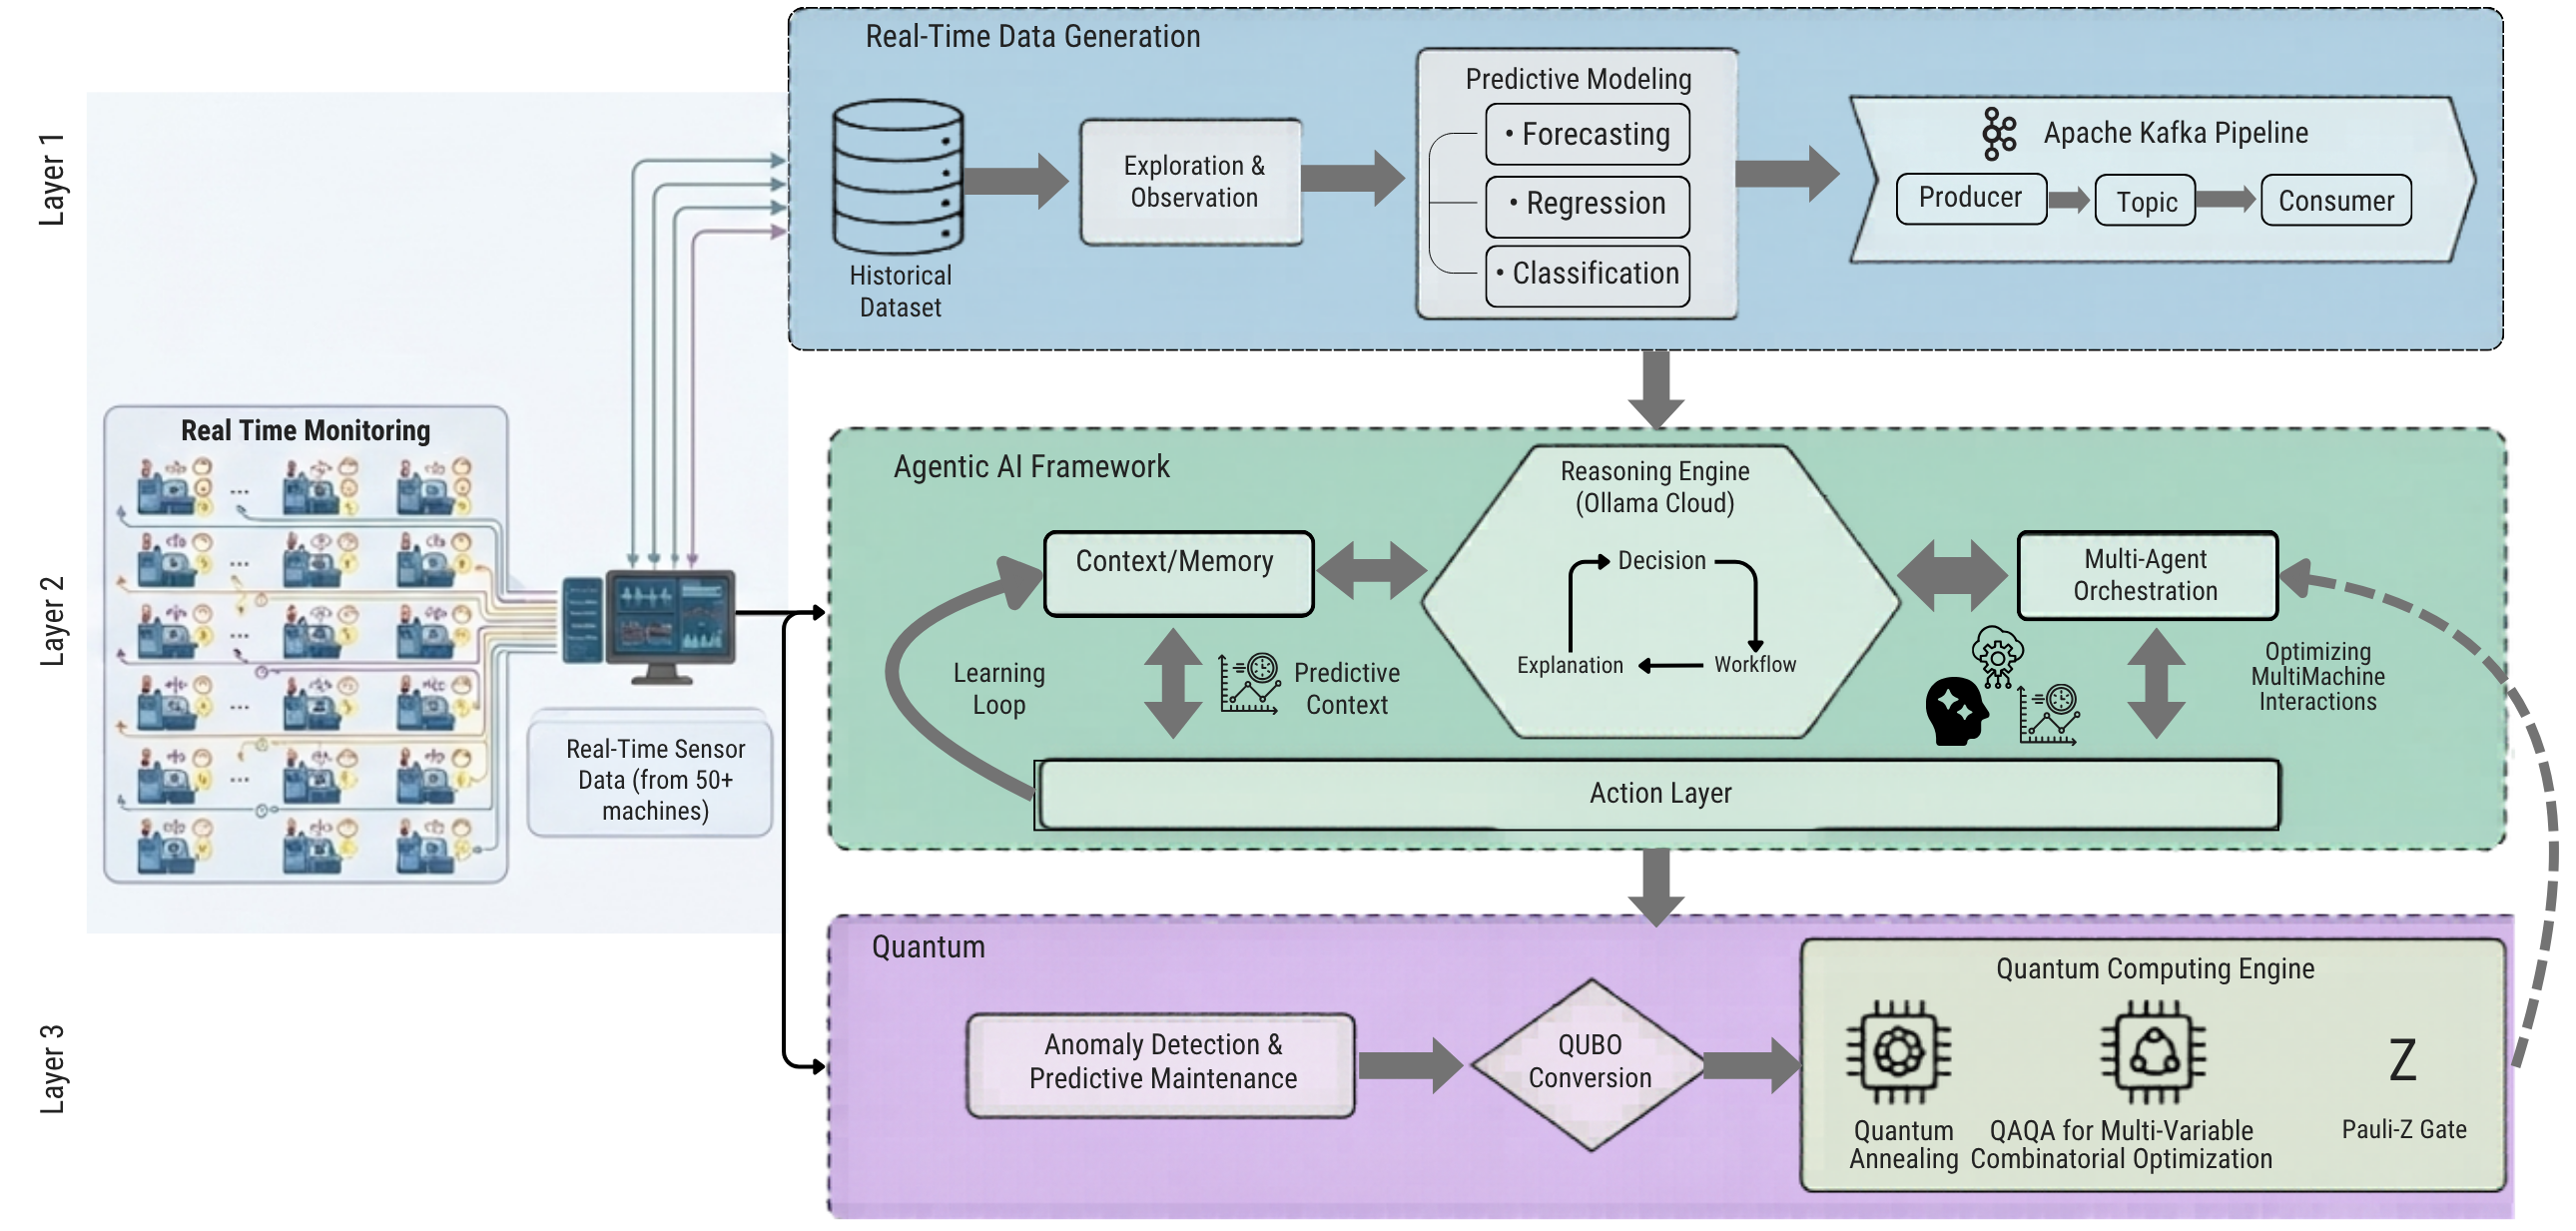
\includegraphics[width=1\textwidth]{figures/images/Research Methodology - Comprehensive Industrial AI & Quantum Optimization Workflow.png}
    \caption{QASAMAP three-layer research methodology architecture.}
    \label{fig:research_methodology}
\end{figure}
\subsection{Smart Manufacturing Setting}

A central enabling concept in modern smart manufacturing is the \textbf{digital twin}, a virtual replica of a physical asset, process or system that synchronizes with real-world data in near real time. The digital twin paradigm integrates three core components: a \emph{physical space} comprising the actual machines, sensors, and production lines; a \emph{virtual space} containing simulation models, physics-based representations, and data-driven predictors; and a \emph{data link} that continuously streams sensor measurements, operational states, and environmental conditions from the physical to the virtual space, enabling bidirectional feedback \cite{Zhao2019}. In predictive maintenance, the digital twin serves as the computational substrate on which anomaly detection, remaining useful life estimation, and maintenance scheduling are executed without disrupting live production.

% \begin{figure}[!htbp]
%     \centering
%     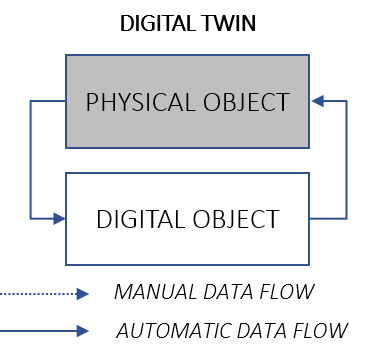
\includegraphics[width=0.6\textwidth]{figures/images/digital_twin_dataflow.png}
%     \caption{Digital Twin data flow architecture in manufacturing. Adapted from Kritzinger (2018).}
%     \label{fig:digital_twin_method}
% \end{figure}

The QASAMAP framework instantiates the digital twin concept through its layered pipeline. Layer~1 ingests streaming sensor events from the physical machine pool and mirrors them into the T-GCN forecasting model and supervised prediction ensemble within the virtual space. Layer~2's agentic orchestration system reasons about the virtual representation---anomaly scores, RUL predictions, and failure type classifications---rather than requiring direct access to the physical machines. Layer~3's quantum-inspired heuristics operate on the digital twin's abstract risk state, scheduling maintenance actions that are then dispatched back to the physical factory floor through the action executor. This closed-loop digital-twin architecture ensures that all predictive maintenance intelligence is computed on a synchronized virtual replica, minimizing latency and risk to live operations.

The QASAMAP framework is motivated by five convergent research gaps identified through systematic literature review and grounded in the empirical properties of the 100,000-reading smart manufacturing dataset (50 machines, 69 days, January--March 2025). The dataset exhibits 8.92\% anomalous readings, 19.70\% maintenance-required instances, and 16,333 critical low-RUL cases (1,637 below 10 hours), illustrating the scale and urgency of accurate maintenance prediction. The five gaps are: \textbf{Gap~1} is the siloed treatment of anomaly detection, prognostics, and scheduling as separate problems \cite{Chalapathy2019, pang_deep_2021, Gao2022}. \textbf{Gap~2} is the classical intractability of machine-level maintenance scheduling across large machine pools \cite{Blekos2024, symons_practitioners_2023}. \textbf{Gap~3} is the adoption of static model architectures that cannot adapt to non-stationary industrial environments \cite{lee_autoencoder-based_2024}. \textbf{Gap~4} is the limited application of quantum-enhanced risk encoding to industrial sensor assessment \cite{kreplin_squlearn_2025}. \textbf{Gap~5} is the absence of integrated agentic orchestration that simultaneously achieves autonomous decision-making, quantum integration, interpretability, and continuous learning \cite{ouyang_llmsense_2024, xing_deepsqa_2021}. QASAMAP addresses all five gaps within a single closed-loop framework.

\subsection{Data Sources and Characteristics}

The dataset models a smart manufacturing environment where machines are continuously monitored using industrial sensor variables. Each machine observation includes physical sensor readings and derived maintenance labels. The main physical variables are temperature, vibration, humidity, pressure, and energy consumption~\cite{widartha_smart_lighting_2024}. These variables describe the operational state of a machine and serve as inputs for anomaly detection, remaining useful life estimation, risk scoring, and maintenance planning~\cite{widartha_hiper_chad_2025}.

The selection of these channels and the design of the sensing environment build on prior sensor-driven monitoring studies. Widartha et al.~\cite{widartha_smart_lighting_2024} showed, in a smart-lighting energy-management setting, that fusing direct sensing-device measurements with an external data source under a rule-based decision layer optimises real-time operation more effectively than any single source alone. QASAMAP applies the same principle: the five raw channels are fused with engineered cross-sensor features and a heuristic decision layer rather than being modelled in isolation. The treatment of the resulting multivariate stream is further informed by the HIPER-CHAD model of Widartha and Kim~\cite{widartha_hiper_chad_2025}, which separates the temporal modelling of normal behaviour from the probabilistic modelling of prediction uncertainty: a recurrent network forecasts the next reading and a variational autoencoder learns the distribution of the resulting residual errors. This prediction-error perspective motivates QASAMAP's forecasting-first design, in which the T-GCN of Layer~1 supplies the expected sensor trajectory against which deviations are scored.

\begin{table}[htbp]
\centering
\caption{The historical CSV dataset summary}
\label{table:dataset_summary}
\begin{tabularx}{\textwidth}{lX}
\hline
Property & Value \\
\hline
Number of records & 100,000 \\
Number of machines & 50 \\
Records per machine & approximately 2000 \\
Minimum records per machine & 1906 \\
Maximum records per machine & 2092 \\
Start timestamp & 2025-01-01 \\
End timestamp & 2025-03-11 \\
\hline
\end{tabularx}
\end{table}


The historical dataset contains 100,000 records collected from 50 machines over the period from 2025-01-01 to 2025-03-11. Each record represents one machine condition observation, including sensor measurements, machine status, anomaly indicator, predicted remaining useful life, failure type, downtime risk, and maintenance requirement. The streaming dataset is produced by a digital twin simulation and stored through a Kafka-MongoDB pipeline. The historical dataset is used for model development, feature analysis, risk formulation, and validation, while the Kafka streaming data is used to evaluate anomaly detection and predictive maintenance in a real-time decision-making scenario.

\begin{table}[htbp]
\centering
\caption{The Feature Description of Historical Dataset}
\label{table:feature_description}
\begin{tabularx}{\textwidth}{l l X}
\toprule
Feature & Type & Description \\
\midrule
Timestamp & datetime & Observation time of the machine vent \\
Machine\_id & categorical / integer & Unique machine identifier \\
Temperature & continuous & Machine temperature reading \\
Vibration & continuous & Machine vibration level \\
Humidity & continuous & Environmental humidity near machine \\
Pressure & continuous & Pressure reading from machine/system \\
Energy consumption & continuous & Machine energy usage \\
Machine status & categorical & Machine state code \\
Anomaly flag & binary & Indicates whether anomaly is detected \\
Predicted remaining life & continuous & Estimated remaining useful life \\
Failure type & categorical & Type of detected or predicted failure \\
Downtime risk & continuous/binary & Estimated risk of downtime \\
Maintenance required & binary & Whether maintenance is required \\
\bottomrule
\end{tabularx}
\end{table}


Table~\ref{table:dataset_summary} summarizes the key properties of the historical CSV dataset, and Table~\ref{table:feature_description} describes each feature column.

The empirical consequences of siloed modelling are directly observable in the dataset. The anomaly flag, predicted RUL, failure type, and maintenance required label are all statistically interdependent: temperature correlates with anomaly flag at $r = 0.447$, anomaly flag correlates with downtime risk at $r \approx 1.0$, and RUL correlates with downtime risk at $r = -0.436$. The 16,333 readings with RUL below 50 hours represent machines that are simultaneously anomalous and prognostically critical a dual characterization that joint modeling exploits far more effectively than independent models.



